
\subsection{Analyse myticket}
Bei myticket ist die Verteilung der Fehler wieder breiter. Es wurden mehr Kriterien verletzt, aber die Anzahl der Fehler ist geringer.

Auch hier sind einige Kontrastfehler aufgetreten. Es sind zwar nicht so viele wie bei Eventim, aber sie machen trotzdem einen großen Teil der Fehler aus. 

\begin{figure}[H]
    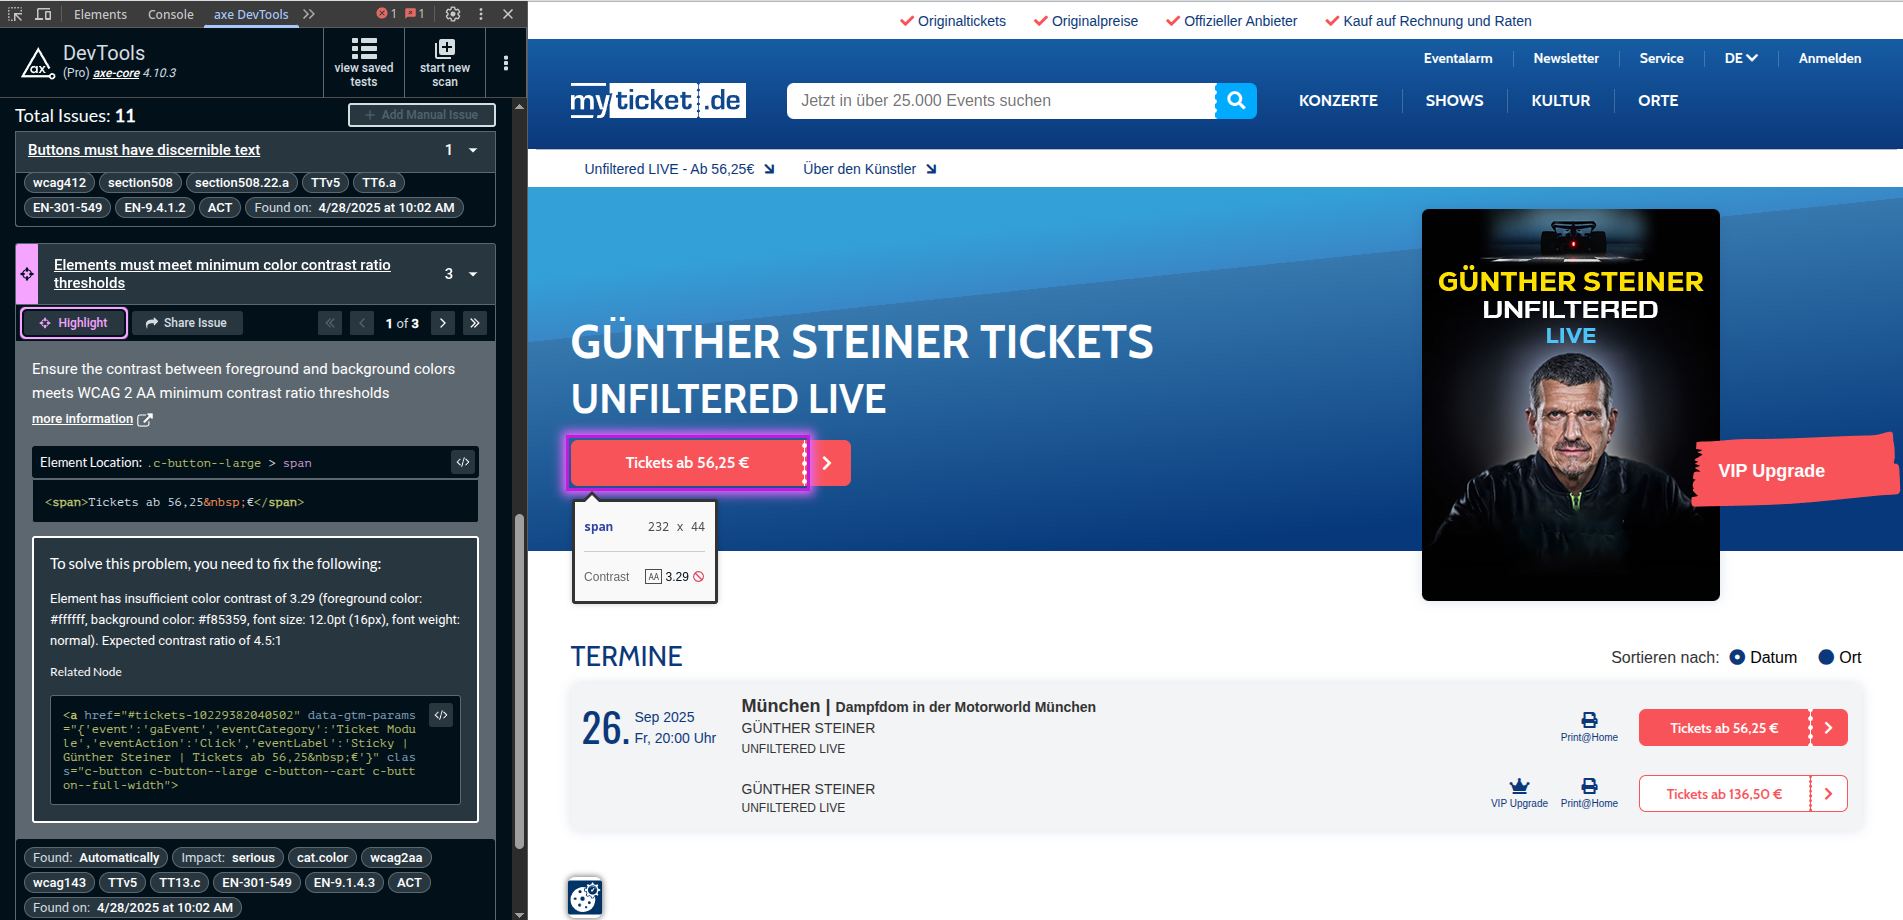
\includegraphics[width=\textwidth]{img/myticket_failed-minimum-contrast.png}
    \caption{Kontrastprobleme auf der Startseite}
\end{figure}

Am häuftigsten wurde das Kriterium 2.4.7 \enquote{Fokus sichtbar} verletzt. Auch hier wurde der Fokus manuell getestet und ist auf vielen Elementen nicht vorhanden.

Danach folgt das Kriterium 2.4.4 \enquote{Link Zweck} und 4.1.2 \enquote{Name, Rolle, Wert}. Dabei handelt es sich um Links, die keinen zugänglichen Namen haben.

\begin{figure}[H]
    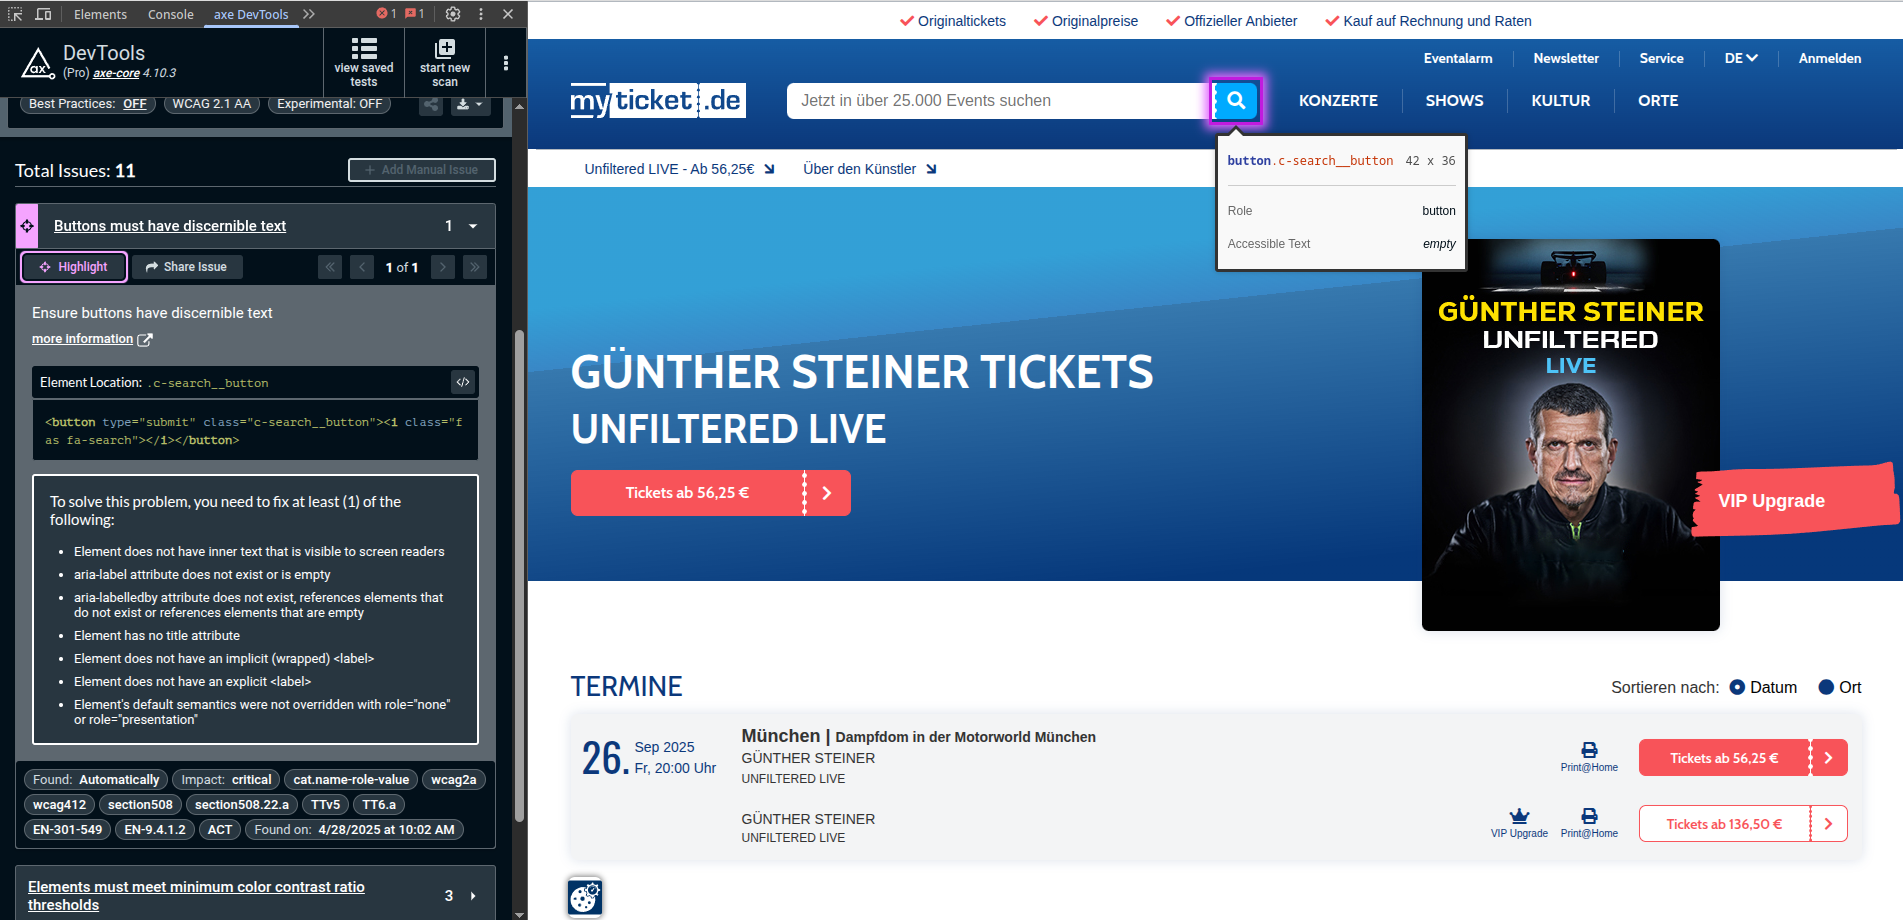
\includegraphics[width=\textwidth]{img/myticket_button-no-accessible-text.png}
    \caption{Fehlendes Label bei einem Button}
\end{figure}

\begin{figure}[H]
    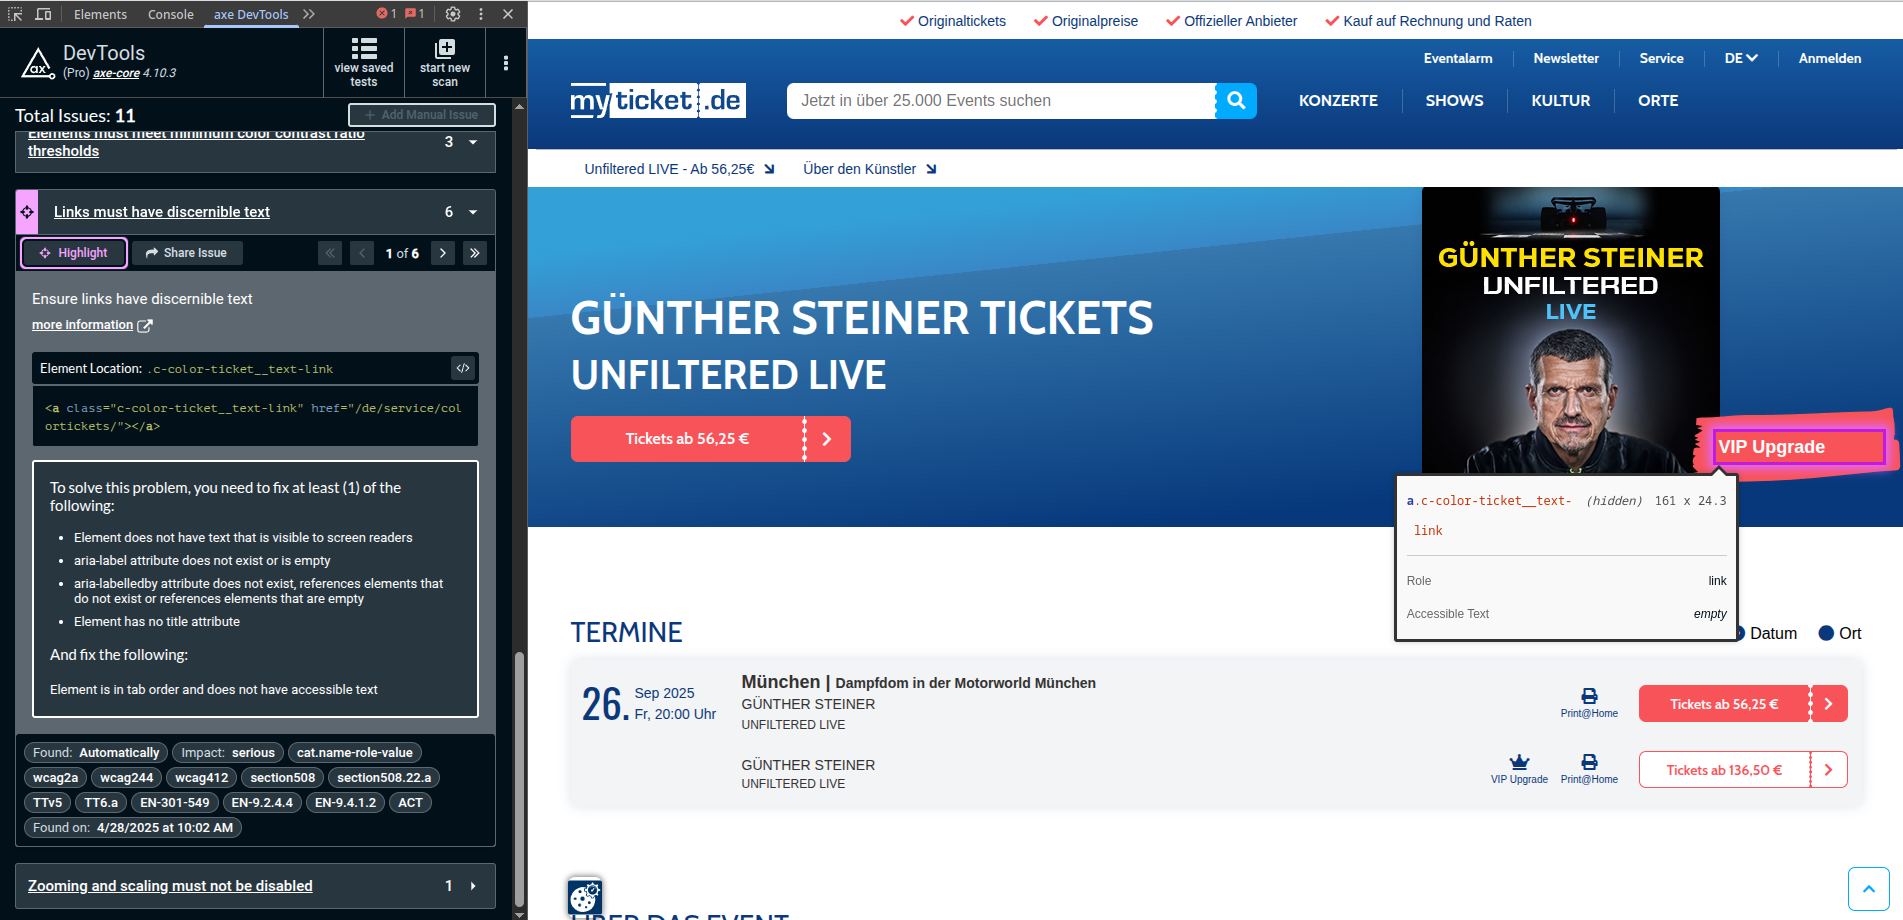
\includegraphics[width=\textwidth]{img/myticket_link-no-accessible-text.png}
    \caption{Fehlendes Label bei einem Link}
\end{figure}

In der Summe sind einige Fehler aufgetreten. Im Vergleich zu Eventim sind die Fehler aber breiter über die Kriterien verteilt. Auch hier sind die Kontrastfehler nicht so häufig wie bei Eventim, aber trotzdem noch vorhanden.

\begin{figure}[H]
\begin{tikzpicture}
\begin{axis}[
    width=\textwidth,
    height=10cm,
    ybar,
    bar width=12pt,
    xlabel={WCAG-Kriterium},
    ylabel={Fehleranzahl},
    symbolic x coords={ 9.1.1.1, 9.1.3.1, 9.1.4.3, 9.1.4.4, 9.2.4.1, 9.2.4.4, 9.2.4.6, 9.2.4.7, 9.3.3.2, 9.4.1.2 },
    xtick=data,
    x tick label style={rotate=45, anchor=east},
    ymin=0,
    ymax=350,
    enlarge x limits=0.1,
    legend style={cells={anchor=west}, legend pos=north east},
    nodes near coords,
    nodes near coords style={font=\scriptsize},
]
\addplot table[x=WCAG-Kriterium,y=Fehleranzahl_axe,col sep=tab]{csv/output/wcag_analyse_myticket_xxxx.csv};
\addplot table[x=WCAG-Kriterium,y=Fehleranzahl_WAVE,col sep=tab]{csv/output/wcag_analyse_myticket_xxxx.csv};
\legend{axe,WAVE}
\end{axis}
\end{tikzpicture}
\caption{Auswertung Analyse myticket}
\end{figure}
